\chapter{Use case}\label{ch:usecase}
To illustrate the simplicity of the library we implemented a use case, called \textit{Plateforme DD}. The goal was to visualize the links between the content of the website\footnote{https://sciences.brussels/dd/}. The visualization and functionality is completely different than the one for GuideaMaps and can be seen in figure \ref{fig:plateforme-dd}.\\

\begin{figure}[H]
	\centering
	\frame{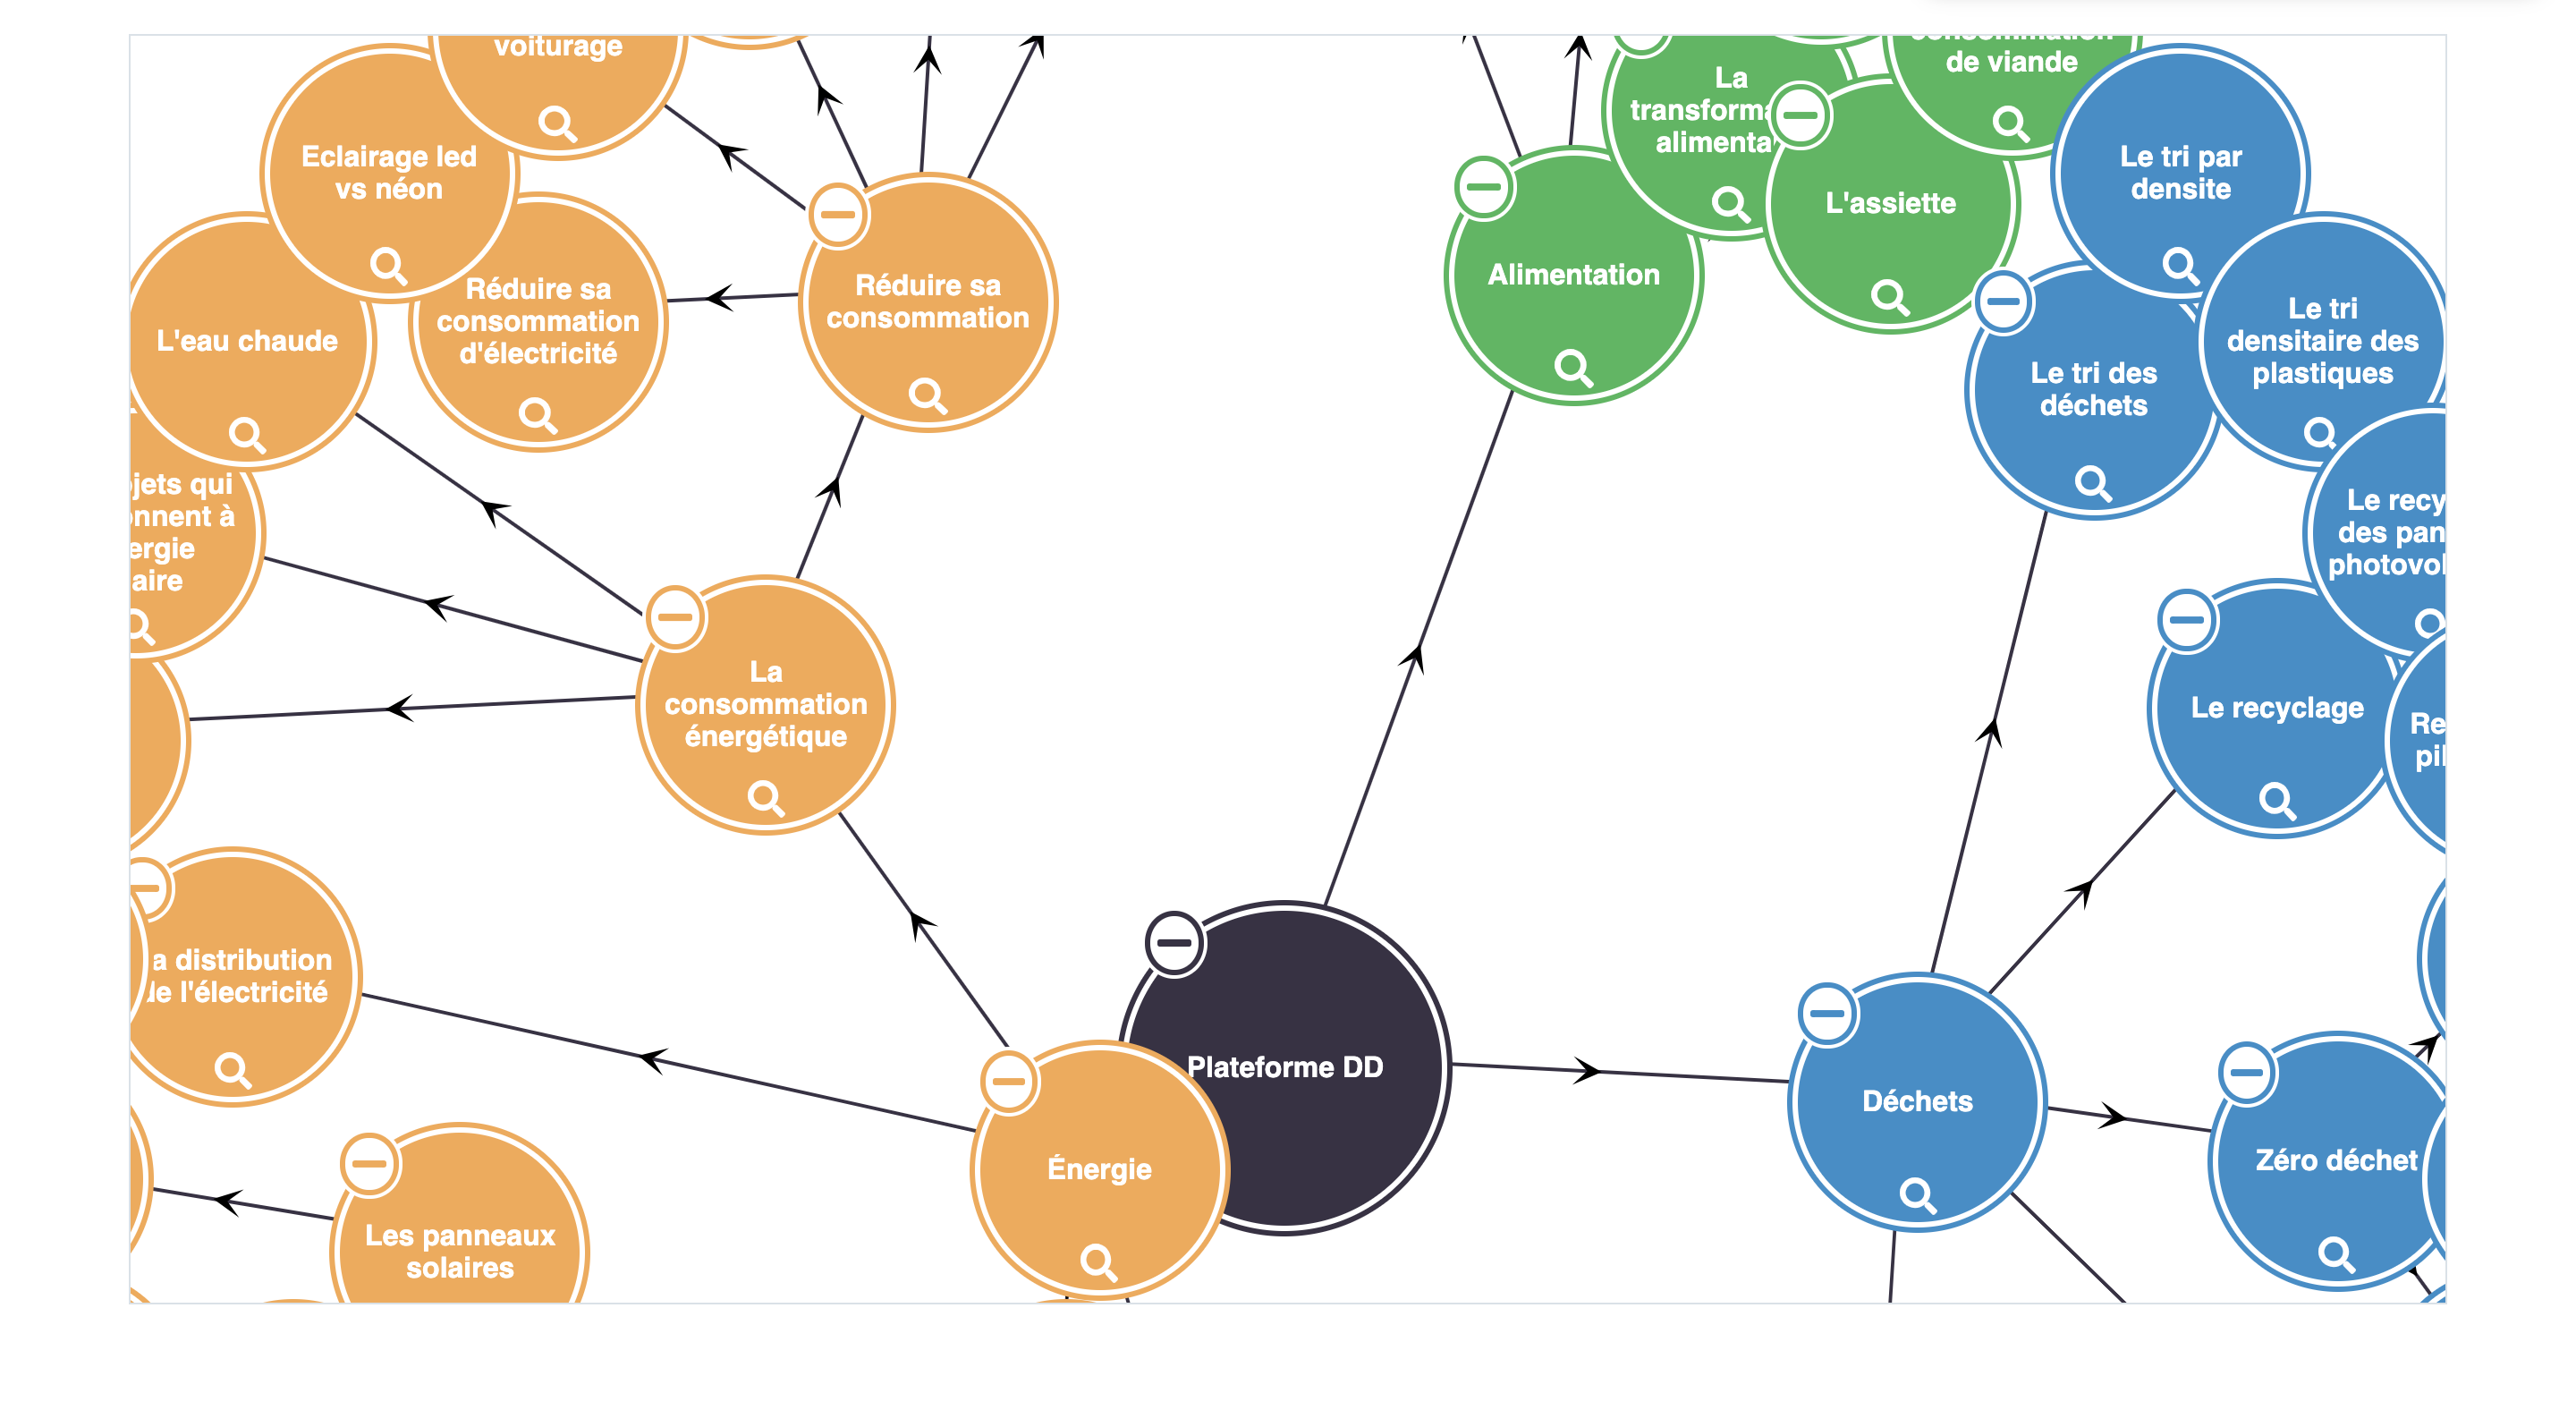
\includegraphics[width=\linewidth]{plateforme-dd.png}}
	\caption{Plateforme DD Layout.}
	\label{fig:plateforme-dd}
\end{figure}

The most obvious difference, which can immediately be seen, is the layout of the nodes. In GuidaMaps, we had rectangular nodes, while in Plateforme DD the nodes are circular. 